\section{Part III: Why ``Workspace + Skill'' Is the Key Leap}
\headingnote{From Tool Use to Reusable Digital Work}

The preceding parts describe two necessary but incomplete advances: stronger cognitive cores and more capable tool-using agents.
This part argues that the next qualitative leap comes from combining reusable skills with persistent workspaces.
A workspace defines the durable environment in which an agent works: files, terminals, browsers, repositories, logs, memories, permissions, and execution contexts where task state persists, as illustrated by OpenClaw-style workstation agents and software-engineering platforms \citep{openclaw2026repo,wang2024openhands,yang2024sweagent,angulodelafuente2026openclawp2p,huo2026abotclaw,weidener2026agentonly,shuolucs2026awesomeopenclawresearch,vardanyan2025building}.
A skill defines how an agent repeatedly performs a class of work: reusable procedures, scripts, examples, checks, dependencies, and safety constraints that turn one-off instructions into operational knowledge \citep{wang2023voyager,anthropic2026skillsdocs,openclaw2026skillsdocs,ling2026agentskills,qihang2026llms,thomasmultimodal,wang2025openhands,sannia2025design,gong2025secure}.
Together, they transform LLM systems from answering models or tool-calling agents into digital workers that inherit procedures, operate in bounded environments, and deliver verifiable outcomes \citep{jimenez2023swebench,xie2024osworld,theagentcompany2024,marro2025permission,kulonen2026model,chrysochos2026society,tang2026workspace,sharma2026contextcov,pan2024training,xia2025live,wang2024agent,zhang2024autocoderover,mundler2024swt,liu2024marscode}.
We therefore develop this thesis through two complementary dimensions: workspace as the execution substrate for agentic work, including the delegation patterns through which users authorize and supervise that work, and skills as reusable procedures for workspace-based agents.


\begin{figure}[t]
    \centering
    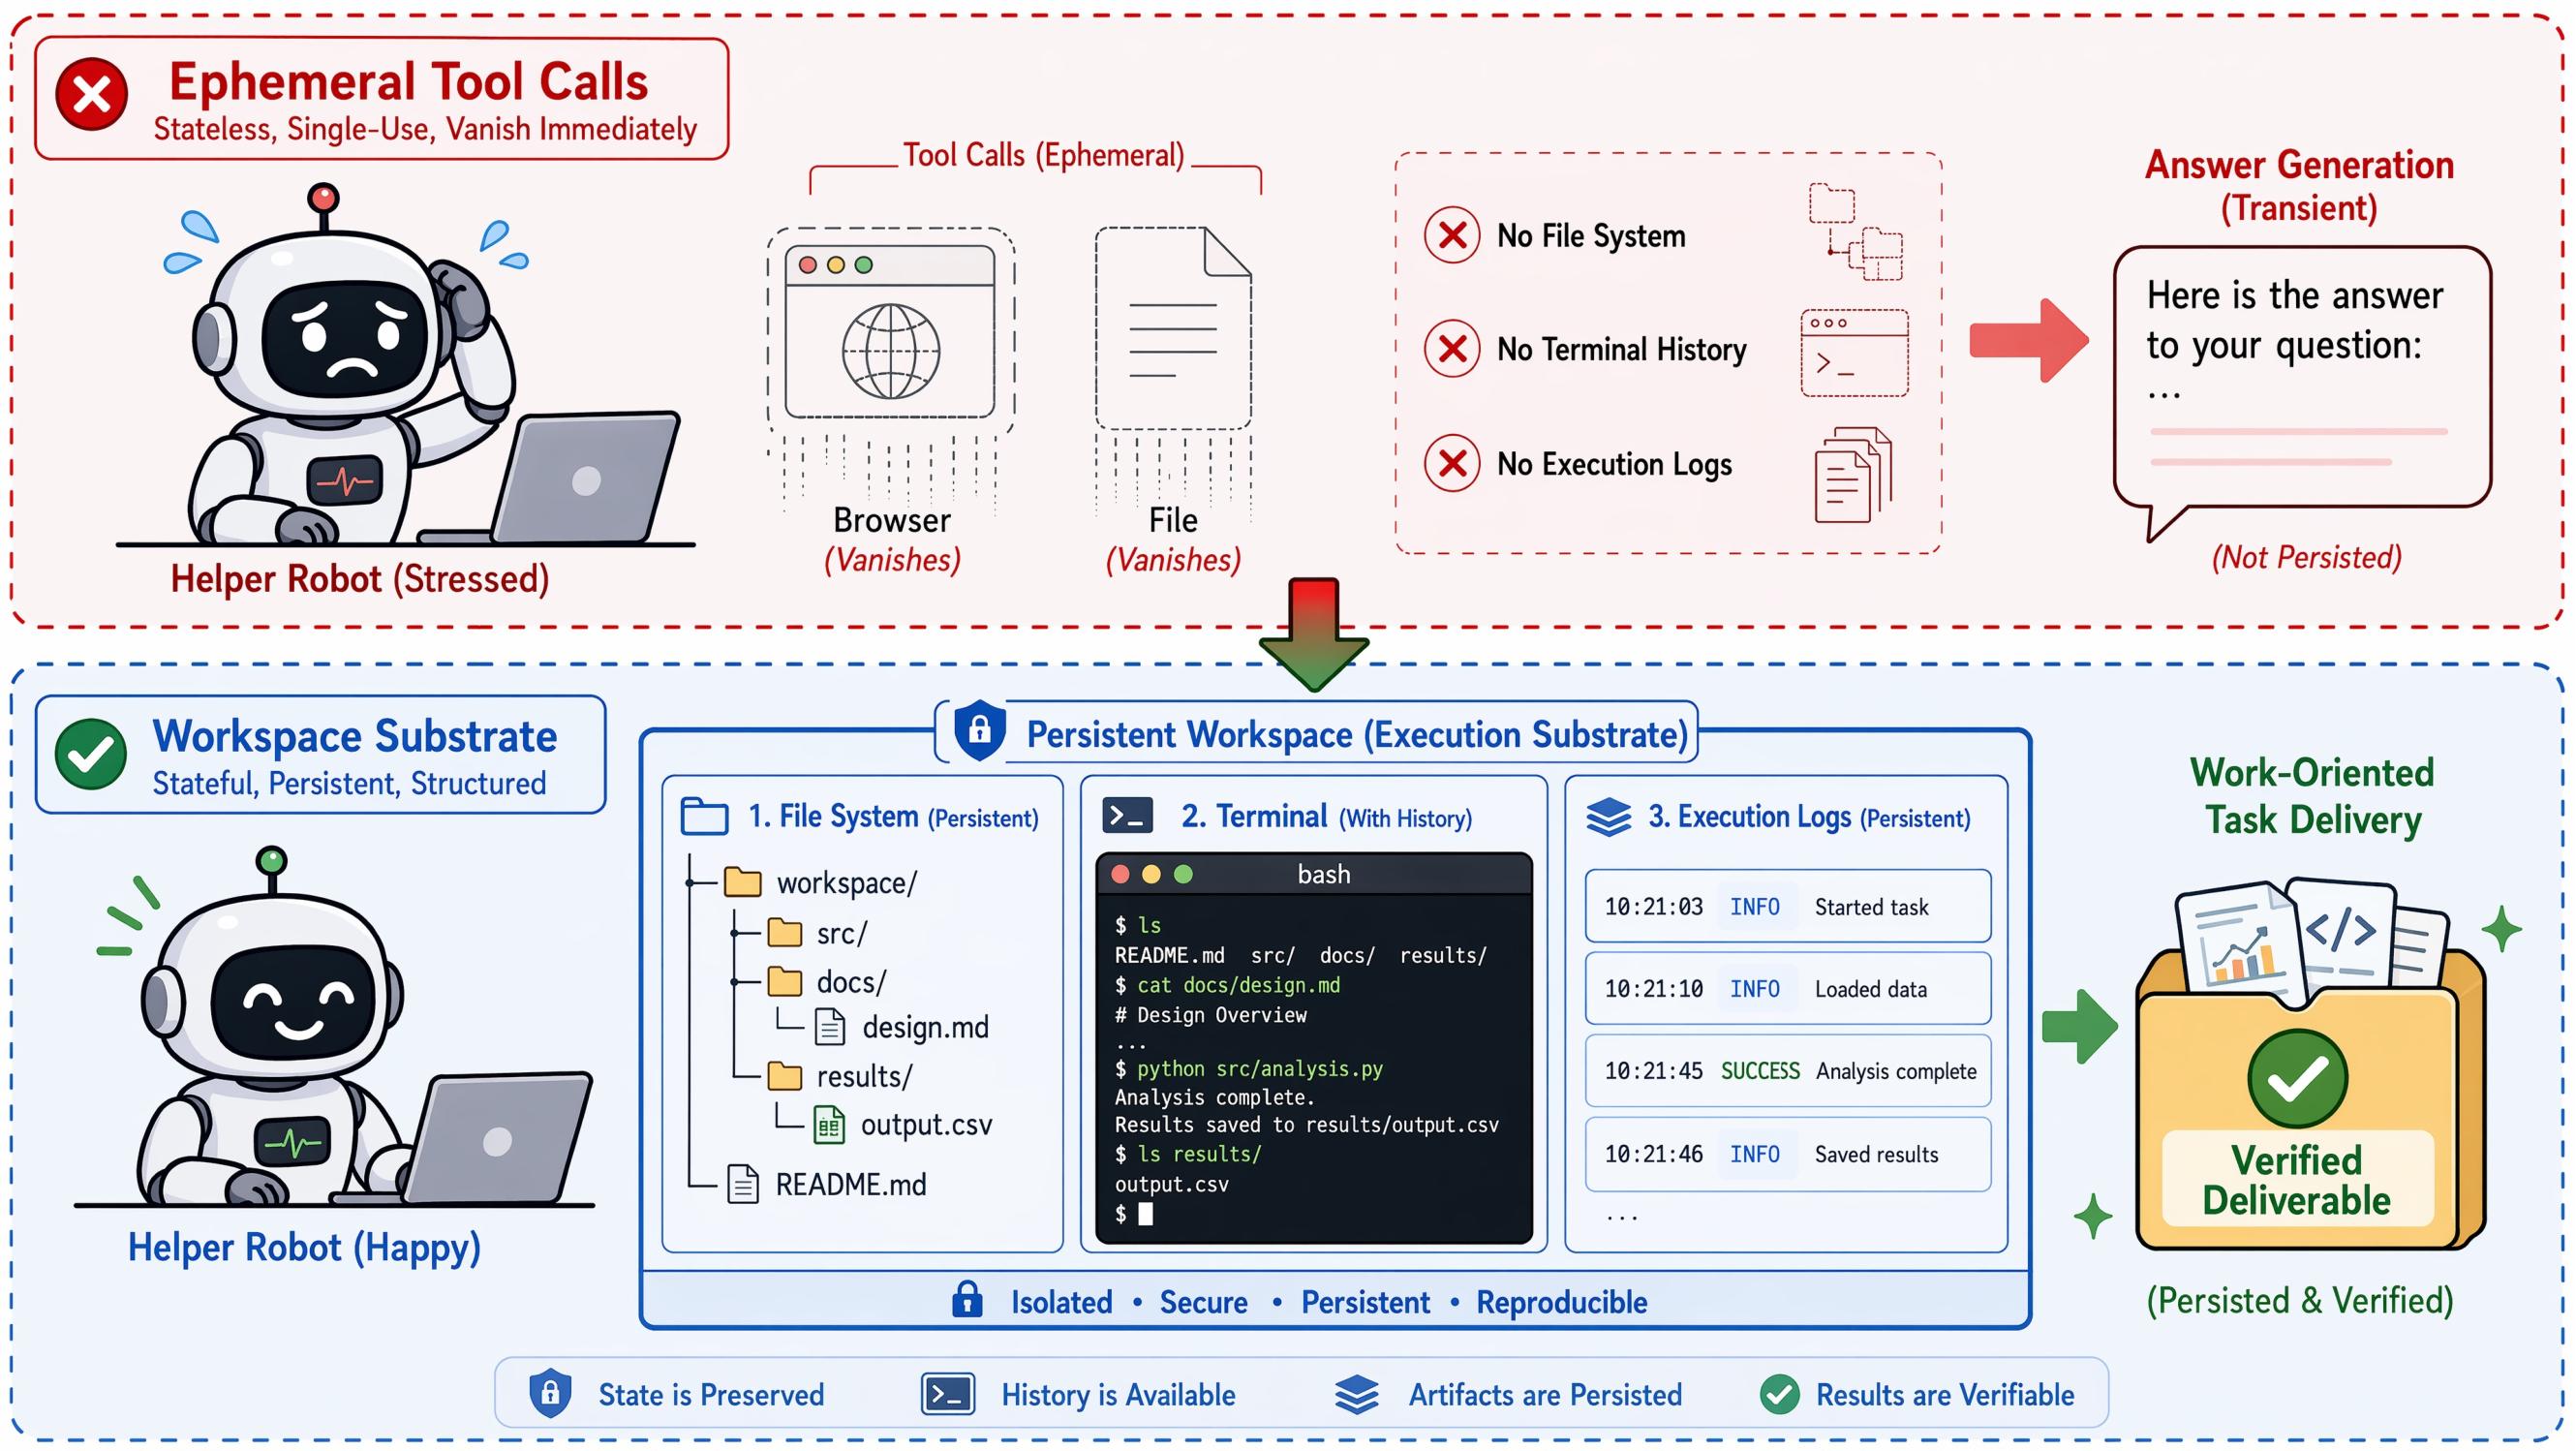
\includegraphics[width=\textwidth]{figure/tool.pdf}
    \caption{Simple tool invocation: the LLM can call external tools to handle local sub-tasks, but these calls remain limited when the task requires persistent files, terminal sessions, execution logs, intermediate artifacts, and recoverable state. The figure highlights why a workspace is needed to support more complex, long-horizon task completion beyond isolated tool calls.}
    \label{fig:tool}
\end{figure}

\subsection{Workspace as the Execution Substrate for Agentic Work: Stateful Context for Tasks}
\headingnote{Persistent environments for durable task delivery}

As shown in Figure~\ref{fig:tool}, the interactive workspace represents the first half of this paradigm leap because complex real-world work cannot be reduced to isolated, stateless API calls. While earlier generation agents could invoke tools, isolated tool invocation alone does not provide system continuity, process inspectability, or state recoverability. In contrast, executing complex long-horizon work requires a persistent, stateful environment where generated artifacts can safely survive, failures can be diagnosed, failed commands can be rerun, and final workspace states can be rigorously inspected \citep{openclaw2026repo,wang2024openhands,yang2024sweagent,suwansathit2026security,fotopoulos2026specialized,hu2025agentsentinel,ge2023llm,wu2025git}. This subsection explains why the workspace becomes the execution substrate that turns agentic behavior from episodic action into durable task delivery.

\subsubsection{From Ephemeral Tool Calls to Persistent State}

Tool APIs give agents the ability to affect the external world, but they do not by themselves provide a stable place for work to accumulate.
When each tool call is treated as an isolated transaction, the agent must repeatedly reconstruct context from limited observations, allowing small inconsistencies to compound across long trajectories~\citep{zhang2025ufo2,oliviero2llm,adam2026towards,buhler2025securing,piao2025agentbay}.
A persistent workspace changes this by giving the agent durable state: editable files, persistent terminals, browser history, versioned repositories, process logs, and local memory for task context \citep{openclaw2026repo,wang2024openhands,yan2025fault,dong2026deltabox,meng2025cellmate,laiqopenclaw,aravind2026agentwall}.
The result is a shift from calling tools around the model to embedding the model inside an environment where work has continuity over time.
In this setting, the important question is no longer only whether the agent can choose the right next action, but whether the environment after many actions remains coherent, inspectable, and recoverable~\citep{eykholt2026lessons,wang2025openhands,zhong2026don,roman2026orchestral,patel2026beyond}.

This change also clarifies why workspace-level design is not merely an engineering detail.
A workspace determines which state is visible to the agent, which operations are executable, which artifacts persist, and which traces can be audited after failure.
It therefore shapes the agent's practical intelligence as much as the underlying model does in deployment.
For software tasks, for instance, the gap between a stateless code-generation prompt and a workspace with editable files, tests, terminals, dependency managers, and version control is the gap between plausible code and repairable engineering task completion \citep{yang2024sweagent,jimenez2023swebench,chancoding,chen2026skillcraft,xu2026agent,cai2024large,shi2025tool}.
For knowledge work, the same distinction appears in document editing, data analysis, project coordination, and research assistance: useful work needs artifacts that can be opened, revised, checked, and handed off~\citep{chen2026cua,lumer2026tool,liupolicy,paranjape2023art,gantayat2026dfagent}.
Persistent workspace is therefore the material substrate of task closure.

\subsubsection{From Answer Generation to Authorized Work Delegation}

Human professional work is rarely a single input-output mapping.
It involves preparing context, following procedures, coordinating diverse tools, checking intermediate results, documenting decisions, and handing off deliverables.
The Workspace + Skill paradigm imports this structure into complex digital environments: the agent does not merely answer questions, but joins a workflow with state, process, accountability, and completion criteria~\citep{huang2026raw,zhang2026formal,zhangkeeps,chen2024t,zhang2026evoagent}.
This reframes next-generation AI systems as work-oriented systems whose performance depends on how well they model and execute the structure of real work.
The evaluation target consequently shifts from mere textual plausibility to task delivery: whether the final workspace state satisfies the user's intent and whether the process can be inspected \citep{xie2024osworld,zhou2023webarena,drouin2024workarena,theagentcompany2024,niu2024screenagent,naveen2025command,liu2024large,sheng2024language,chatlatanagulchai2025agent}.

Once agents inhabit persistent workspaces, the dominant human--AI interaction pattern also shifts from instruction to delegation.
In the chatbot setting, interaction is primarily instructional: the user writes a prompt, the model returns an answer, and correction happens through another prompt.
For workspace-based agents, the user no longer specifies every micro-step, but delegates a bounded objective together with constraints, permissions, success criteria, and acceptable risk.
The interface must therefore support task scoping, authority assignment, progress monitoring, intervention, and final acceptance, not only message exchange.
This turns the agent from a reactive respondent into a collaborative worker whose actions are evaluated through both its final artifacts and the trajectory that produced them \citep{xie2024osworld,drouin2024workarena,theagentcompany2024,marro2025permission}.

This delegation pattern changes what humans need to observe.
In command-style interaction, the user mainly inspects the next textual answer.
In authorized collaboration, the user instead watches process summaries, reasoning states, tool actions, file diffs, execution logs, checkpoints, unresolved assumptions, and the evolving workspace state.
Human control shifts from continuously telling the model what to do next toward granting authority, adjusting constraints, interrupting unsafe or unproductive paths, and auditing whether the final state satisfies the delegated intent.
The system must decide what authority the agent has, where execution boundaries are drawn, which actions require confirmation, how failures are rolled back, and how responsibility is recorded.
Different tasks can therefore adopt different autonomy levels: direct instruction for short reversible actions, supervised delegation for medium-risk multi-step work, and conditional autonomy for well-specified procedures with strong verification and rollback.
The key interaction unit is no longer a single response, but an inspectable work episode in which intent, authority, action, observation, verification, and accountability are jointly represented \citep{openclaw2026repo,wang2024openhands,li2026prism,zhao2026clawguard,gruber2026agenticforensics}.
In this setting, competition between AI systems shifts from raw tool coverage to delivery quality: whether the agent completes work reliably, safely, and transparently under realistic constraints \cite{reliability2026computeruse,rabanser2026sciencereliability,rosset2026verifiers}.
Workspace design therefore becomes inseparable from governance design, because persistence enables task closure while also determining how actions can be constrained, audited, and recovered \cite{wang2026openclawsec,li2026prism,zhao2026clawguard,gruber2026agenticforensics}.

\begin{AIbox}{Key Shift: From Tool Calls to Delegated Workspaces}
    \begin{itemize}[left=2pt,topsep=1pt,itemsep=2pt, parsep=1pt]
        \item Atomic tool calls allow an agent to act, but they do not preserve enough state for long-horizon work to remain coherent, inspectable, or recoverable.

        \item Persistent workspaces provide durable files, terminals, logs, repositories, and execution contexts, turning episodic actions into verifiable task delivery.

        \item Delegation interfaces expose authority, progress, intermediate reasoning state, and final workspace state so that humans can supervise work without specifying every micro-step.
    \end{itemize}
\end{AIbox}

\subsection{Skills for Workspace Agents: Reusable Procedures for Repeatable Work}
\headingnote{Procedural memory for repeatable workspace execution}

As shown in Figure~\ref{fig:workspace}, skills are the procedural half of the leap because a persistent workspace alone does not explain how agents accumulate reusable operational knowledge.
Prompts describe what the user wants in a particular moment, but skills encode how a system should repeatedly perform a family of tasks.
A useful skill can package procedural instructions, scripts, examples, dependencies, verification checks, rollback strategies, and safety constraints \cite{wang2023voyager,anthropic2026skillsdocs,anthropic2026skillsrepo,openclaw2026skillsdocs,openclaw2026skillsrepo}.
This subsection explains how skills turn ad-hoc instruction following into reusable capability packages, and why their value becomes fully visible only when they are executed inside persistent workspaces.


\begin{figure}[t]
    \centering
    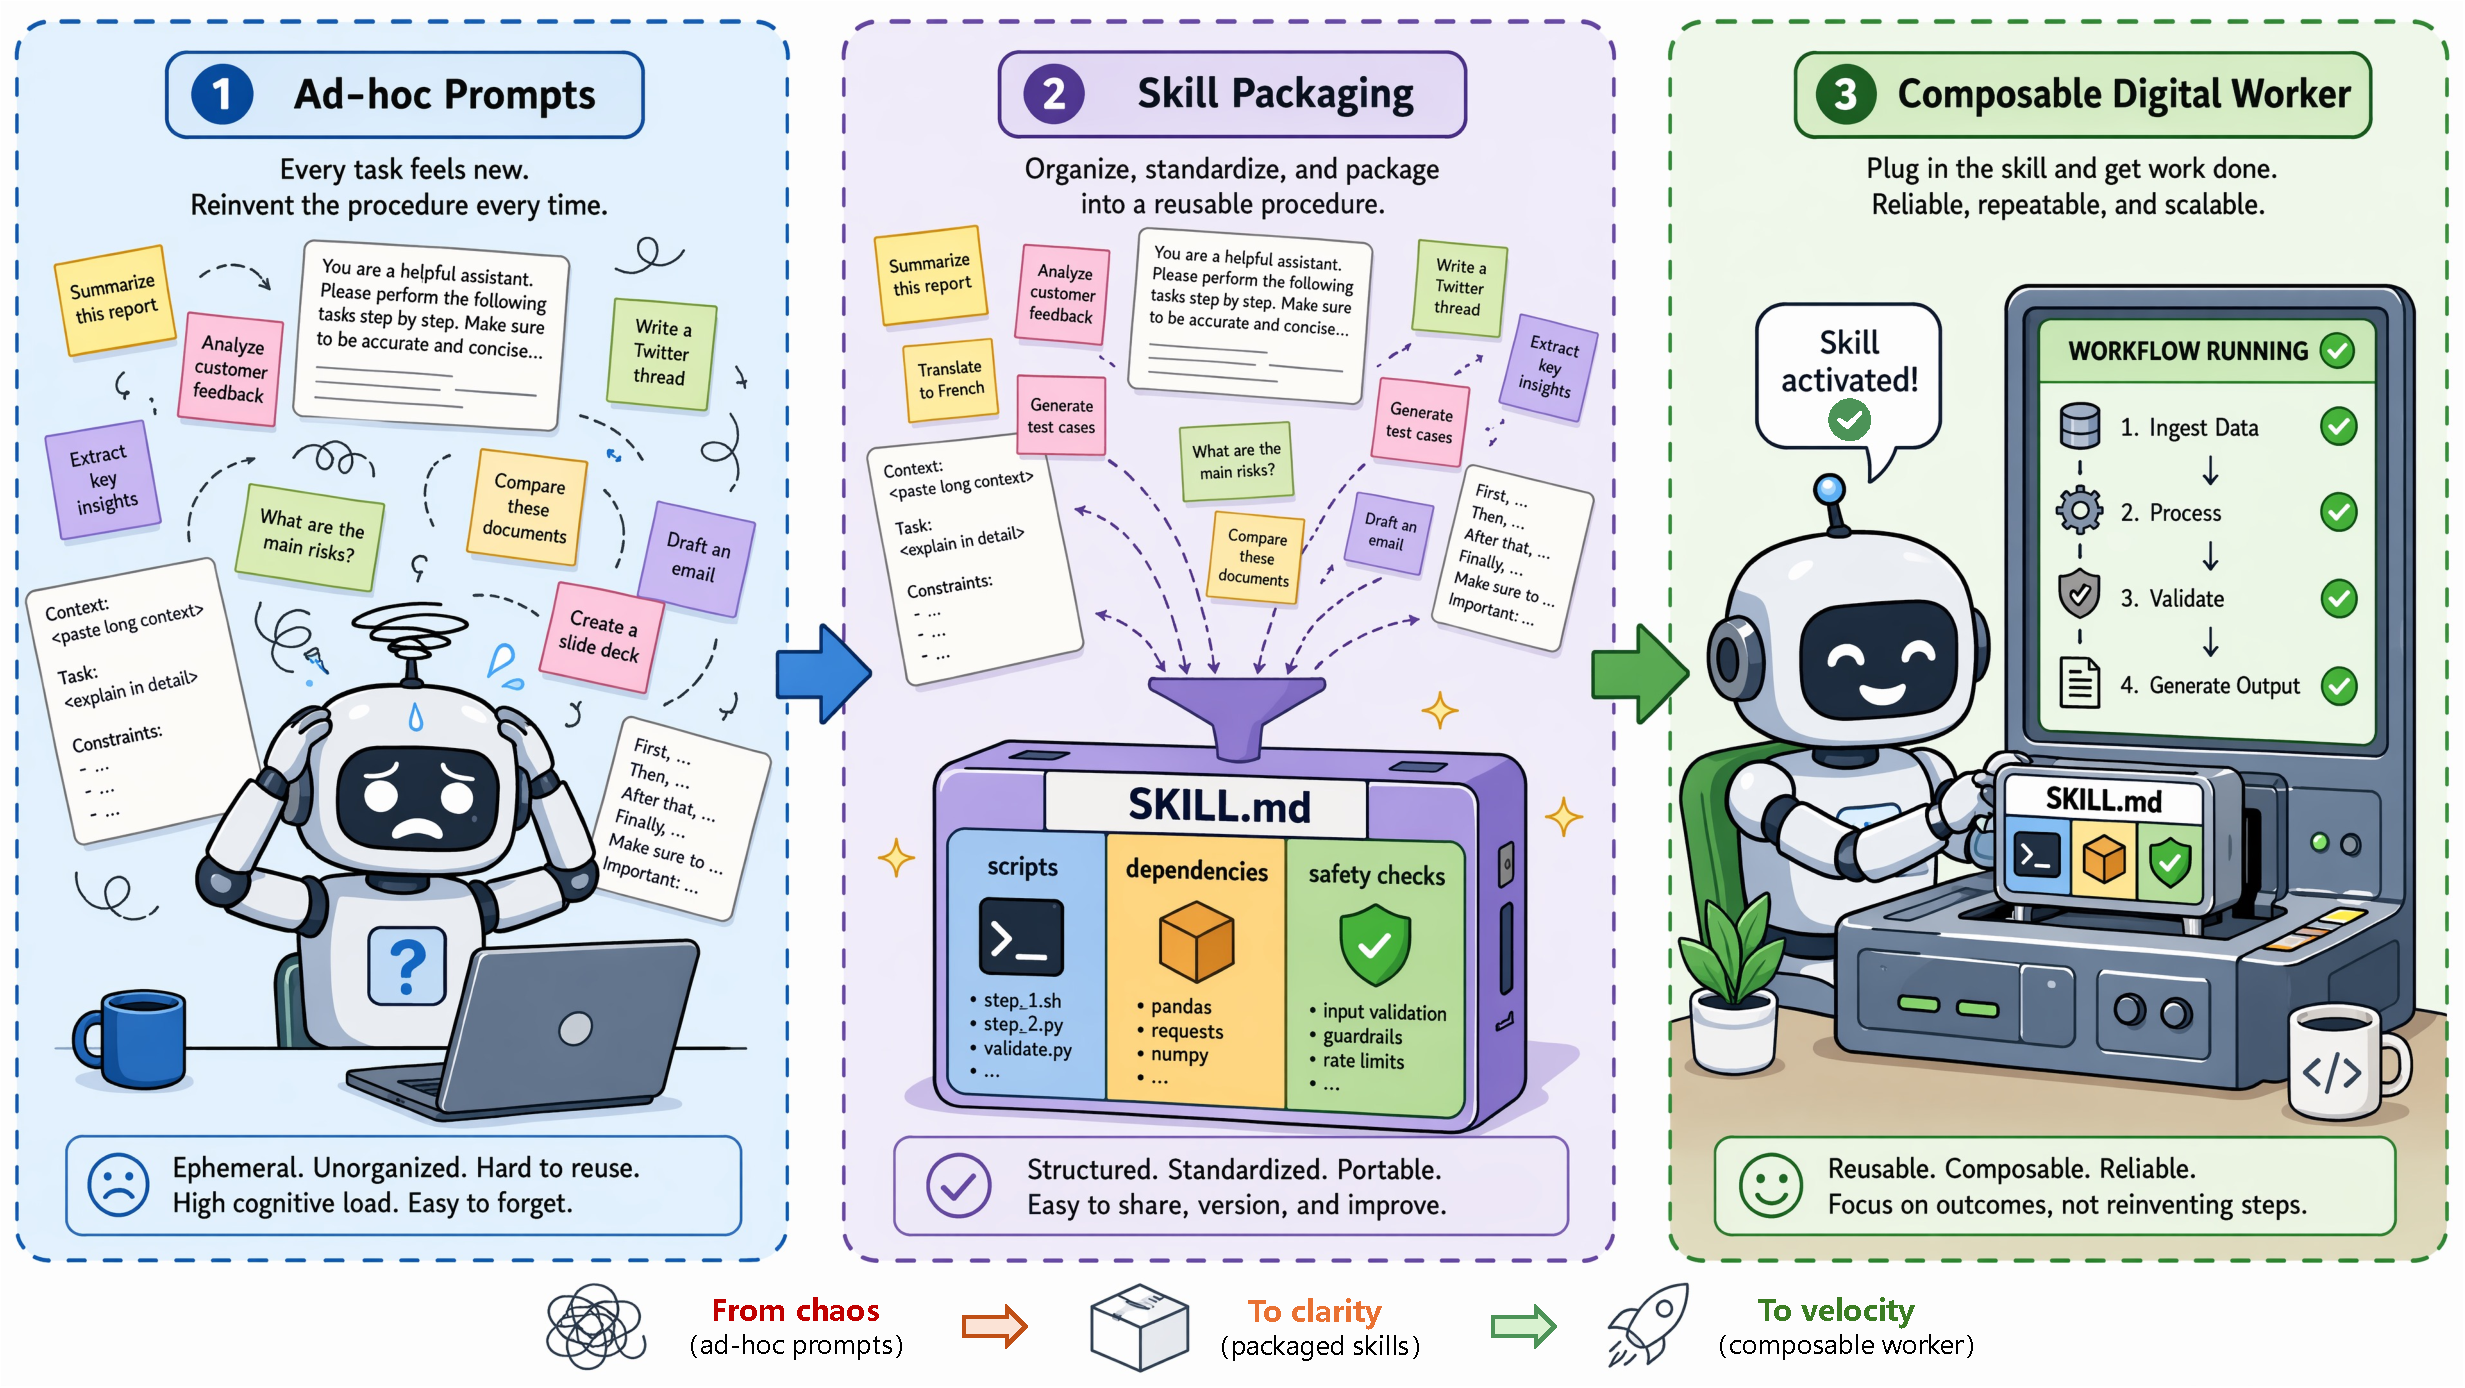
\includegraphics[width=\textwidth]{figure/workspace.pdf}
    \caption{Workspace + Skill paradigm: persistent workspaces provide the stateful place where work happens, while skills package reusable procedures, scripts, checks, and safety constraints. The figure shows how agents combine workspace context with skill assets to produce verifiable digital work instead of one-off responses.}
    \label{fig:workspace}
\end{figure}


\subsubsection{From Ad-hoc Prompts to Composable Capability Packages}

Prompts are temporary and local: they guide a single interaction, but they rarely become durable assets that can be tested, versioned, reused, or governed. As complex tasks become longer and more specialized, repeatedly encoding all relevant procedures in the prompt becomes inefficient and unreliable. Skills address this limitation by externalizing procedural knowledge into modular reusable packages. Instead of asking the model to rediscover a task each time, a skill provides a detailed recipe for a task family, including tools, inputs, steps, failure modes, validation criteria, and safety constraints \cite{anthropic2026skillsdocs,openclaw2026skillsdocs}. This changes capability accumulation from transient prompt engineering into a maintainable asset layer outside the pretrained model weights \cite{wang2023voyager,ling2026agentskills}.

The key advantage of such skills is their composability. A skill can be parameterized for different projects, combined with other skills, refined through experience, and inspected by expert humans before reuse \cite{anthropic2026skillsdocs,openclaw2026skillsrepo,ling2026agentskills}. It can also contain executable components, such as scripts or templates, that reduce unnecessary dependence on fragile natural-language reasoning. In this sense, skills are neither simple prompts nor ordinary tools. They sit between model cognition and workspace execution: they translate task intent into repeatable procedures that the agent can invoke when operating in a concrete digital environment. As skill libraries mature, agent systems can inherit organizational know-how in a form that is modular, reviewable, and portable across tasks.

\subsubsection{From Skill Libraries to Integrated Digital Workers}

Modular skills become most powerful when coupled with persistent workspaces. The workspace provides state, context, tools, and artifacts; the skill provides procedure, constraints, and verification logic. A skill without a workspace risks remaining a static instruction template, while a workspace without skills forces the autonomous agent to improvise repeatedly. Their combination enables stronger task closure: the agent can load a reusable procedure, operate over persistent artifacts, check results, repair failures, and leave an inspectable final state \cite{openclaw2026repo,wang2024openhands,jimenez2023swebench}. This is the point at which an LLM system begins to resemble a digital worker rather than an assistant.

OpenClaw provides a concrete lens because it combines a persistent local environment, skill directories, tool integrations, and task-oriented execution in one unified architecture \cite{openclaw2026repo,openclaw2026skillsdocs,openclaw2026skillsrepo}. Rather than treating OpenClaw as a single isolated product, we use it as a representative example of a broader system pattern: a model is wrapped by a harness that manages workspace state, loads reusable procedures, routes actions through tools, and exposes the resulting work process to evaluation and governance. This pattern shows why competition among next-generation autonomous AI systems is not merely about more tools or larger models, but about transforming reusable procedures into reliable, bounded, inspectable work \cite{reliability2026computeruse,rosset2026verifiers,bhardwaj2026skillfortify}. In this view, the Workspace + Skill paradigm is the bridge from agentic capability to practical delivery-grade AI labor: skills define reusable ways of working, while workspaces make those ways reliably executable, verifiable, and accountable.

\paragraph{Case study: OpenClaw as a Workspace + Skill system.}
OpenClaw illustrates how the Workspace + Skill paradigm can be translated from an abstract design principle into a concrete computational workstation architecture. At the workspace layer, the system exposes persistent files, local project context, terminals, browsers, tool integrations, communication channels, logs, and task-specific instructions to the autonomous agent \cite{openclaw2026repo}. These components give the model a bounded digital worksite rather than a simple collection of disconnected API calls. A task can therefore leave intermediate artifacts in the file system, reuse command outputs, preserve verifiable execution evidence, and support later inspection by users or evaluators. This workspace substrate is what allows the agent to move from producing a plan to actually changing a target environment.

At the skill layer, OpenClaw follows the emerging pattern of packaging reusable procedures as directory-level assets, often centered around a \texttt{SKILL.md} file and accompanied by scripts, resources, examples, dependencies, and operational instructions \cite{openclaw2026skillsdocs,openclaw2026skillsrepo,voltagent2026awesomeopenclawskills}.
Such a skill is more than a prompt because it can encode preconditions, tool choices, expected intermediate artifacts, validation routines, common failure modes, and safety constraints.
It is also more than a tool because it does not merely expose one callable function; it describes a repeatable way of working inside a workspace.
In this sense, skills function as procedural memory that can be loaded only when relevant, inspected by humans, revised over time, and shared across related task families.

A typical OpenClaw-style execution loop consists of four stages.
First, the system interprets user intent and maps it to the workspace state, including available files, tools, permissions, and context.
Second, it retrieves or activates relevant skills that provide procedural guidance for the task family.
Third, it executes actions inside the workspace, producing observable state changes such as edited files, command outputs, browser states, or generated artifacts.
Finally, it verifies whether the final state satisfies the task objective, using tests, file diffs, logs, state inspection, or human confirmation when necessary.
The key point is that the unit of intelligence is no longer a single response but the combined trajectory of skill selection, workspace operation, verification, and recovery.

This case study clarifies why delivery-grade agents require governance at the same level as capability.
Because OpenClaw-style systems can operate over local files, external services, credentials, and third-party skills, their reliability depends on permission boundaries, provenance tracking, sandboxing, audit logs, and rollback mechanisms \cite{li2026prism,zhao2026clawguard,gruber2026agenticforensics}.
The same architecture that enables task closure also amplifies the consequences of wrong actions.
Therefore, OpenClaw should be seen not only as an example of more capable tool use but as a broader shift toward managed work execution: persistent environments and reusable skills must be paired with verification and runtime control.

\begin{AIbox}{Key Difference: Skills as Operational Memory}
    \begin{itemize}[left=2pt,topsep=1pt,itemsep=2pt, parsep=1pt]
        \item Prompts specify immediate intent, but they rarely become reusable assets that can be tested, versioned, governed, and applied across repeated task families.

        \item Skills package procedures, scripts, checks, and safety constraints so that workspace-based agents can convert reusable know-how into accountable digital work.
    \end{itemize}
\end{AIbox}

\paragraph{Limitations of the Workspace + Skill paradigm.}
Although Workspace + Skill is a useful lens for understanding next-generation agentic systems, it should not be interpreted as a complete solution to reliable autonomy.
The paradigm improves continuity and reuse, but it also introduces new failure modes at the level of skills, workspaces, and their interaction.
A balanced view is therefore necessary: persistent environments and reusable procedures can raise the ceiling of agentic work, but they also increase the need for lifecycle management, security review, and operational discipline \cite{Pezeshkpour2026FromTS,Li2025SAFEFLOWAP}.

\textbf{Skill brittleness and environmental drift.}
In practice, skills are often written for particular tools, file layouts, APIs, software versions, permission settings, and organizational conventions.
When any of these conditions change, a previously useful reusable skill may silently become invalid.
For example, a browser workflow can break after a UI redesign, a command-line skill can fail after a minor dependency update, and an API-oriented skill can produce incorrect downstream actions after a schema change.
This makes skill maintenance an ongoing requirement rather than a simple one-time authoring problem.
Robust skill systems therefore typically need versioning, dependency declarations, compatibility checks, regression tests, and deprecation mechanisms \cite{bhardwaj2026skillfortify,Aghazade-Par2025FeatureBasedFL,Yaroshynskyi2025InvestigatingTE}.

\textbf{Skill overfitting and negative transfer.}
Reusable procedures can also become too specialized.
A skill that encodes a highly specific workflow may perform well in the environment where it was created but mislead the autonomous agent in a slightly different target workspace.
This creates a form of procedural overfitting: the system mechanically follows a familiar recipe even when the current task requires adaptation.
Negative transfer is especially risky when skill retrieval is entirely automatic, because the agent may load an irrelevant or partially relevant skill and anchor subsequent planning on inappropriate assumptions \cite{Jiang2023ForkMergeMN,Meftah2021OnTH}.
Future systems must therefore evaluate not only whether a skill succeeds on its original task family, but also when it should not be invoked.


\textbf{Workspace contamination and state inconsistency.}
Persistent digital workspaces preserve useful context, but they also preserve stale files, failed intermediate artifacts, obsolete logs, corrupted caches, and misleading partial outputs.
Unlike a simple stateless prompt, a workspace can accumulate noise across time.
If the autonomous agent cannot distinguish authoritative artifacts from accidental leftovers, persistence may reduce rather than improve reliability.
This problem becomes harder in collaborative or multi-agent settings, where several agents may modify shared files, update memory, or operate on overlapping resources.
Workspace hygiene, state summarization, provenance labeling, snapshotting, and rollback are therefore central to making persistence trustworthy \cite{Li2025SAFEFLOWAP,Zheng2025LifelongAgentBenchEL}.

\textbf{Security and supply-chain risk.}
Skills can contain natural-language instructions, executable scripts, dependencies, credentials, assumptions, and tool permissions.
They present a supply-chain attack surface.
A malicious or poorly reviewed skill may exfiltrate data, request excessive authority, modify files unexpectedly, or steer the model toward unsafe tool use.
Similarly, a compromised workspace can poison the agent through files, web pages, tool outputs, or memory entries.
Therefore, skill registries and workspace agents require provenance tracking, permission manifests, sandboxed execution, user confirmation for high-risk actions, and continuous audit trails \cite{li2026prism,zhao2026clawguard,wang2026openclawsec,Jia2026SkillJectEA,Liu2026ExploitingLA,Liu2026AgentSI}.

\textbf{Governance overhead and evaluation cost.}
Finally, the practical benefits of Workspace + Skill come with substantial engineering overhead.
Reliable deployment requires not only stronger language models, but also controlled environments, reproducible state snapshots, verifier scripts, permission policies, logging infrastructure, skill tests, and failure recovery procedures.
Evaluation also becomes more expensive because success must be judged over trajectories and final workspace states rather than single responses \cite{Qiang2025MLEDojoIE,Zheng2025LifelongAgentBenchEL}.
Thus, the paradigm shifts the primary bottleneck from prompt design to system operations.
The most successful future systems will likely be those that make this operational layer scalable: skills must be easy to test and share, workspaces must be easy to safely reset and audit, and task closure must be verifiable without excessive manual human intervention.

\begin{AIbox}{Limitation: Reuse Requires Governance}
    \begin{itemize}[left=2pt,topsep=1pt,itemsep=2pt, parsep=1pt]
        \item Workspace + Skill improves task continuity and procedural reuse, but it also introduces brittleness, stale state, negative transfer, and supply-chain risks.

        \item Reliable deployment therefore requires skill lifecycle management, workspace hygiene, permission control, sandboxing, rollback, and trajectory-level evaluation.
    \end{itemize}
\end{AIbox}
